\documentclass{report}
% 导言
\usepackage{xeCJK}
\usepackage{graphicx}
\usepackage{float}
% 加深编号
\setcounter{secnumdepth}{3}
% 正文区
\begin{document}
	% 标题
	\title{通信前言技术}
	\author{Raven}
	\date{}
	\maketitle
	\tableofcontents	
	% 正文
	\chapter{LTE概述}
	\section{LTE性能指标}
	\begin{enumerate}
		\item 数据峰值:上50M,下100M
		\item 延迟: 空闲转活跃100ms,用户面低于5ms
		\item 移动性:速率高达350km/h的用户设备链接
		\item 支持多种带宽分配
	\end{enumerate}
	\section{LTE网络体系架构}
	\subsection{LTE网络体系架构组成}
	\begin{enumerate}
		\item EPS :网络体系的全程
		\item E-UTRAN:演进UMTS陆地无线接入网络
		\item EPC: 演进分组核心网络
	\end{enumerate}
	\begin{figure}[H]
		\centering
		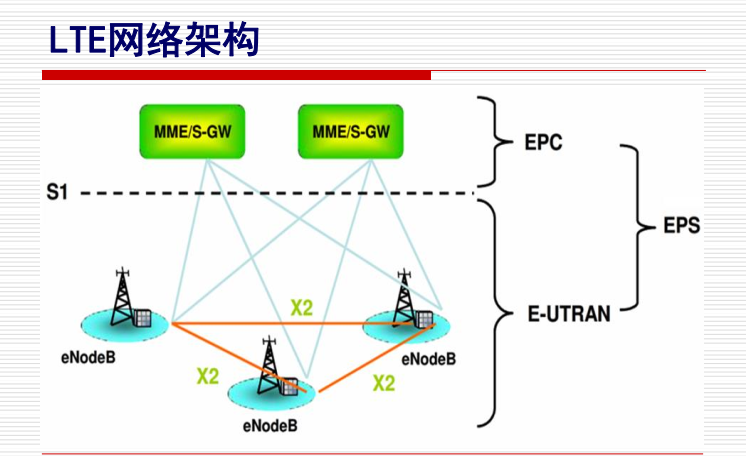
\includegraphics[width=0.7\linewidth]{LTE网络架构}
		\caption{LTE网络架构}
		\label{fig:lte}
	\end{figure}
	\subsection{LTE网络架构特点}
	\begin{enumerate}
		\item 网络结构更加简单扁平
		\item 取消RNC的集中控制,避免单点故障,有利于提高网络稳定性。
	\end{enumerate}
	\section{LTE关键技术}
	\subsection{多天线技术MIMO}
	\begin{description}
		\item[基本概念] 在发送和接收端采用多跟天线,多输入输出
		\item[采用MIMO的目的] 通过充分利用空间资源,提高频谱效率,增加系统容量,实现更广覆盖。
	\end{description}
	\subsubsection{单天线系统容量}
	\begin{figure}[H]
		\centering
		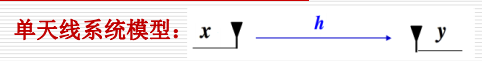
\includegraphics[width=0.7\linewidth]{单天线发射模型}
		\caption{单天线发射模型}
		\label{fig:}
	\end{figure}
	接收端:\(y = xh+n\)。\\
	假设发射段功率为$P_t$,则接收端功率为$|h|^2P_t$。
	接受信噪比$SNR = \frac{P_R}{\sigma^2}=\frac{|h|^2P_t}{\sigma^2}=|h|^2\rho$\\
	信道容量 $C_0 = Blog(1+SNR) = Blog(1+||h|^2\rho)$ \\
	单位频谱信道容量:$C = log(1+|h|^2\rho)$	\\
	\subsubsection{各类系统容量}
	\begin{description}
		\item[SISO] $C = log(1+|h|^2\rho)$
		\item[SIMO] $C = log(1+\sum_{i = 1}^{M}|h|^2\rho)$
		\item[MISI] $C = \frac{1}{N}log(1+\sum_{i = 1}^{N}|h|^2\rho)$
		\item[MIMO] $C = log[det(I_M+\frac{\rho}{N}HH^{*})]$
	\end{description}
	\textbf{在MIMO系统中,如果N,M足够大,$C = min\{N,M\}log(\rho/2)$},其系统容量随着天线数目的增加而线性增加
	\subsection{正交频分复用(OFDM)技术}
	\subsubsection{OFMD实现流程}
	\begin{figure}[H]
		\centering
		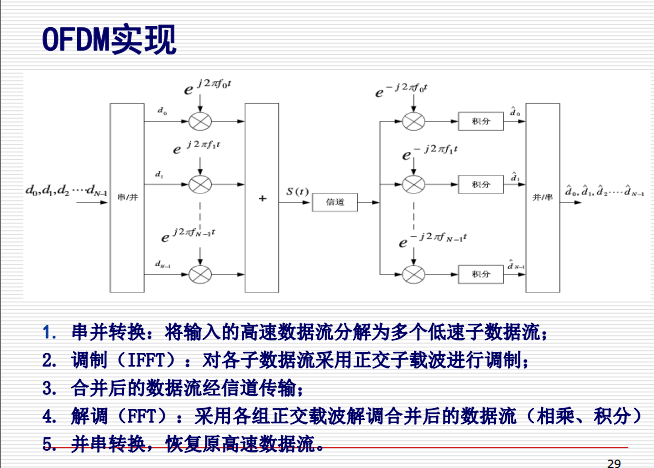
\includegraphics[width=\linewidth]{OFDM实现流程}
		\caption{OFDM实现流程}
		\label{fig:ofdm}
	\end{figure}
	\subsubsection{OFMD的优缺点}
	\begin{description}
		\item[优点] 高频率效率;对抗频率选择性衰落;支持快带传输,消除ISIS影响。
		\item[缺点] 对频率偏移和相位噪声很敏感;峰均比(PAPR)较大,导致射频放大器的功效较低。
	\end{description}
	\section{LTE发展现状}
	发展迅速,\textbf{智能手机}是用户快速增长的主动力。
	\subsection{主要运营商策略}
	\begin{description}
		\item[Verizon
		]  快速建网抢占先机
		\item[DoCoMo] 开放态度对待OTT服务提供商; 为SP用户提供增值服务,实现SP用户快速增加	
		\item[SKT]  快速部署全国性网络
	\end{description}
	\section{LTE发展面临的挑战}
	\begin{enumerate}
		\item 频谱分散
		\item 突发业务的应对
		\item 核心网:网络架构各层之间的感知和保障
	\end{enumerate}
	\section{LTE与4G的关系}
	\subsection{基本概念}
	LTE--3.9G,LTE的演进版本--LTE-Advanced(LTE-A)被称为4G。
	\subsection{性能指标}
	\begin{enumerate}
		\item 	LTE与4G的少量性能存在差异
		\item 4G上行下行峰值速率分别为500Mbps,1Gbps
	\end{enumerate}
	\subsection{关键技术}
	LTE与4G均才用MIMO,OFDM等技术,因此被称为准4G。
	
	\chapter{5G概述}
	\section{5G概念}
	5G是对现有技术的演进,不是一种新技术。
	\subsection{5G标准化进程}
	\begin{enumerate}
		\item \textbf{2016-2018.9}3GPP完成标准制定,满足初步商业化部署。
		\item \textbf{2020}完成全部商业化。
	\end{enumerate}
	\subsection{5G应用场景及性能指标}
	\subsubsection{应用场景}
	\begin{enumerate}
		\item 增强移动带宽(eMBB)。
		\begin{itemize}
			\item 高速上网,办公室,密集住宅。
			\item 更高用户移动性要求。地铁,高铁。
		\end{itemize}
		\item 大规模机器类通信,海量连接(mMTC)。
		\begin{itemize}
			\item 传感和数据采集为目标的物联网场景。环境监测、智能农业、智能家具
			\item  小数据包,传感数据量小。存在大量终端设备。
		\end{itemize}
		
		\item 低时延高可靠通信(URLLC)。场景:智能交通系统(车联网),工业控制等特殊应用需求。指标:毫秒级别。
	\end{enumerate}
	\subsubsection{性能指标}
	\textbf{数据峰值速率,频谱效率,移动性,连接密度,延迟。}
	具体:
	\begin{figure}[H]
		\centering
		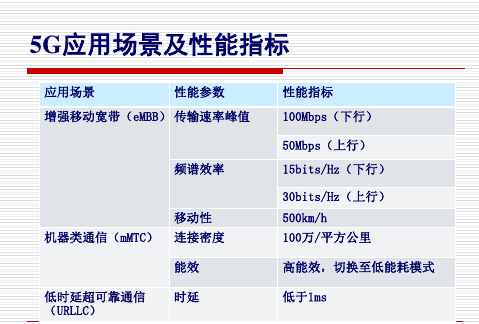
\includegraphics[width=\linewidth]{5G应用场景及性能指.png}
		\caption{5G应用场景及性能指标}
	\end{figure}
	\subsection{5G空口(NR)技术标准进展}
	\subsubsection{码型优化及多址接入}
	\textbf{ 5G将采用基于OFDM优化的波形和多址接入技术
	}
	\subsubsection{灵活的框架设计
	}
	\begin{itemize}
		\item  可扩展时间间隔
		\item  自包含集成子帧
		
	\end{itemize}
	\subsubsection{新型无线技术
	}
	\begin{description}
		\item[大规模MIMO
		]  频谱效率提升、系统容量提高、用户速率及覆盖范围提升
		\item[信道编码技术
		] \textbf{背景:}LTE采用Turbo码作为信道编码方案,但Turbo码译码过程复杂,
		迭代译码方式导致时延过长,不适用于5G应用场景。
		现有码:华为--极化码,高通--LDPC,法国--Turbo2.0
		\item[频谱共享技术] 主要技术LTE-U,LAA(授权辅助接入),MulteFire
	\end{description}
	\subsubsection{终端直连技术}
	讲传统的“终端-网络-终端“的方式变为”终端-终端"
	\textbf{场景}:基础设施无法正常使用的情况。
	
	\textbf{优点:}时延降低、终端能耗降低。
	\subsection{网络架构特点}
	\subsubsection{网络切片}
	\textbf{概念:} 利用虚拟化技术将通用网络基础设施资源虚拟化为多个专用
	虚拟网络,每个虚拟网络称为一个网络切片。
	
	\chapter{移动互联网概述}
	\section{移动互联网概念及特点}
	\subsection{概念}
	移动互联网将移动通信和互联网二者相结合,也即\textbf{用
	户采用移动终端进行网络访问}。
	\subsection{特点}
	\begin{enumerate}
		\item 高便携性 ,随时随地都可使用
		\item 接入便携,可通过多种无线接入技术实现网络访问。
		\item 即时性。
		\item 定向性。基于位置服务
		\item 精准性。个性化。
		
	\end{enumerate}
	\section{移动互联网发展现状}
	使用率最高的是\textbf{即时通信业务},网上购物最多的是\textbf{淘宝}
	\section{移动互联网发展趋势}
	\begin{enumerate}
		\item 实现技术多样化。
		\item 商业模式多元化。
	\end{enumerate}
	
	\chapter{物联网}
	\section{概念和体系架构}
	\subsection{概念}
	物物相连的网络,是互联网的拓展网络。
	\subsection{体系架构}
	\textbf{三层体系架构}:应用层,网络层(各类易构接入网络异构融合),感知层。
	\section{物联网应用}
	\begin{enumerate}
		\item 智能交通
		\item 环境检测
		\item 智能物流
		\item 智能家具
		\item 智能电网
		\item 智能农业
	\end{enumerate}
	\section{物联网发展现状}
	\section{物联网产业链及发展趋势}
	\begin{itemize}
		\item 多元化发展
		\item 与云计算、大数据结合。
		\item 依托蜂窝技术
		\item 微电子成本下降。
	\end{itemize}
	\chapter{云计算}
	\section{定义}
	云计算是一种IT资源的交付和使用模式,提供资源的网络被称为“云”。
	\section{服务形式}
	\begin{itemize}
		\item IaaS:基础设施即服务。租用硬件服务器。
		\item SaaS:软件即服务。租用云服务器。
		\item Pass: 平台即服务。
	\end{itemize}
	\subsection{云类型}
	\begin{itemize}
		\item 公有云,可以用公有云提供个性化的软件。
		\item 私有云,企业自建,为企业专用。
	\end{itemize}
	\section{云计算发展趋势}
	\begin{enumerate}
		\item 虚拟化技术向软硬协同方向发展
		\item  大规模分布式存储技术成为主流技术
		\item  分布式计算技术不断完善和提升
		\item 安全与隐私将获得更多关注
	\end{enumerate}
	\section{云计算应用
	}
	亚马逊 Amazon,谷歌 Google....
	\chapter{ICT行业发展概述}
	\section{ICT发展阶段}
	\begin{enumerate}
		\item 数字化
		\item 信息化
		\item 智能化
		\item 智慧化
	\end{enumerate}
	\section{发展现状}
	\section{技术发展趋势}
	\subsection{CT-传递信息的技术}
	网络重构:核心:云、SDN,NFV与开源。
	\subsubsection{IT-将有用信息进行处理的技术}
	\section{ICT的创新体系}
	“网"创新:聚焦智能网络。
\end{document}